\chapter{Experiments and Results}
\label{cha:experimentsandresults}
%---------------------------------------------------------------------------

\section{Song Popularity}
\label{sec:songpopularity}

The analysis of song popularity provides valuable insights into the factors
that influence the success of music tracks. This problem has two approaches:
\begin{itemize}
  \item \textbf{Regression} - Spotify's popularity is a value on scale of
    0-100. This approach involves training a regression model trying to predict
    that value.
  \item \textbf{Classification} - assigning binary label to the songs(popular
    vs. unpopular) and training a classification model to predict it.
\end{itemize}

In this section the prediction of popularity was attempted using several
regression and classification models. These models were trained on different
sets of features, including Spotify metadata, lyrical attributes, and audio
features, with the aim of investigating the predictive power of those features
and their impact on popularity.

Catboost models were used as the primary predictive tool due to their
robustness and performance in handling complex relationships. 

Baseline models were also implemented to serve as a reference point:
\begin{itemize}
  \item \textit{Baseline Mean Model}: baseline model for regression that always predicts the mean.
  \item \textit{Baseline Majority Model}: baseline model for classification that always predicts the majority class.
  \item \textit{Baseline Random Model}: baseline model for classification that predicts random class.
\end{itemize}

The experiments involved both quantitative evaluatoin and SHAP analysis to
assess feature importance and interpretability of the models.

%---------------------------------------------------------------------------
\subsection{Regression Approach}

\begin{center}
\begin{figure}[H]
  \centering
  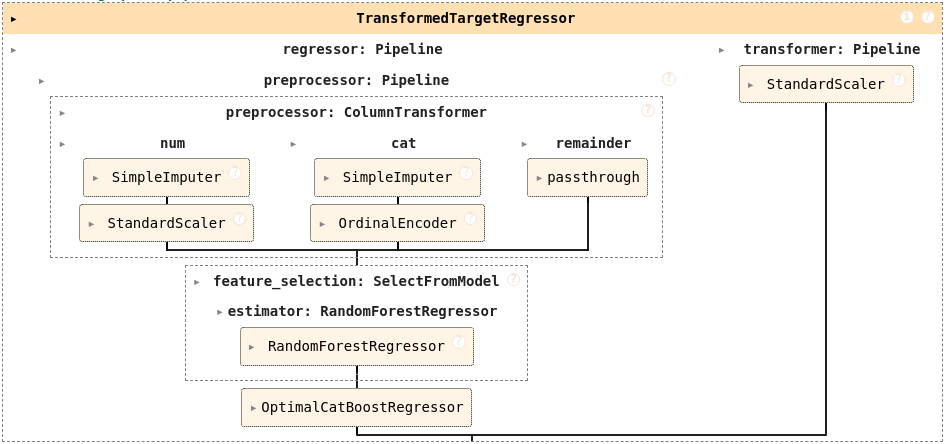
\includegraphics[width=6in]{img/reg_pipeline.png}
  \caption{Regression model pipeline. It involves preprocessing, feature
  selection and CatBoost model.}
  \label{Figure:fig_beh}
\end{figure}
\end{center}

The pipeline was fit with all available features, that includes Spotify audio
features and metadata, lyrical features and features extracted from the audio
files. The feature selection step chose the subset of most valuable features
based on the feature importance from initial Random Forest model.

\begin{table}[H]
\centering
\caption{Results of regression of popularity.}
\begin{tblr}{
  hline{2} = {-}{},
}
 & \textbf{Model}      & \textbf{Features} & \textbf{MAE}  & \textbf{RMSE} & \textbf{$R^2$} \\
 & Baseline Mean Model &                   & 13.53         & 16.90         & -0.01          \\
 & Catboost            & all               & \textbf{6.33} & \textbf{8.52} & \textbf{0.74}  \\
 & Catboost            & lyrical           & 11.81         & 15.29         & 0.17           \\
 & Catboost            & spotify data      & \textbf{6.04} & \textbf{8.10} & \textbf{0.77}  \\
 & Catboost            & audio             & 12.71         & 16.15         & 0.08           
\end{tblr}
\end{table}

As seen in the results table, the CatBoost model trained on spotify data only
achieved the best performance, with \textbf{Mean Absolute Error(MAE) of
\textbf{6.04} and and $R^2$ of 0.77}, closely followed by the model trained on
all features that achieved \textbf{MAE of 6.33 and ($R^2$ of 0.74}. The results
clearly indicate the importance of Spotify audio features and metadata in
prediction of song's popularity. Predicting the success  of a musical track
based on solely the lyrics or acoustic features turned out to be diffifcult and
models trained on those subsets of features showed only slight improvement in
comparison to the baseline model. In contrast, the model trained on Spotify data only
achieved \textbf{55.3\%} better MAE score than the baseline model.

Despite feature selection, the model trained on all features performed slightly
worse than the model trained on Spotify features alone. This likely occurred
because adding less important or redundant features reduced the model's ability
to focus on the most relevant Spotify features. The additional features may
have introduced noise, making it harder to identify clear patterns. This
behavior might also hint at slight overfitting on the redundant features,
despite the use of cross-validation. Increased regularization could potentially
mitigate this issue in future experiments.


SHAP analysis was conducted to interpret the predictions of the regression
model and asses the importance of individual features and their contribution to
song's popularity.


\begin{center}
\begin{figure}[H]
  \centering
  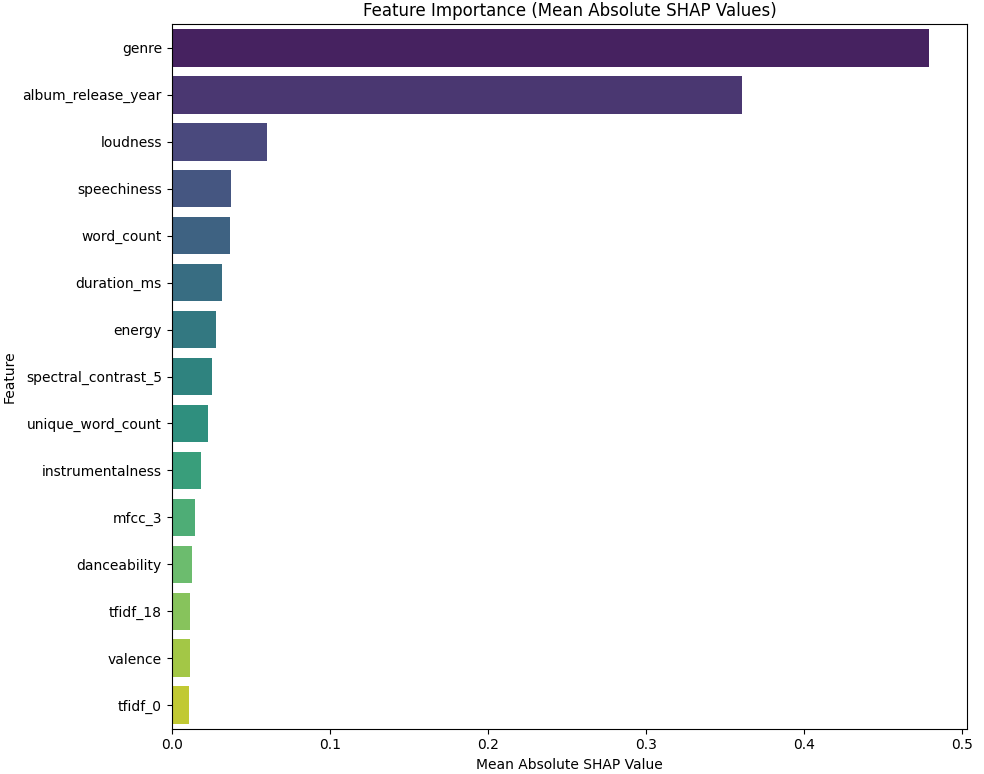
\includegraphics[width=5in]{img/feature_importance_popularity_reg.png}
  \caption{SHAP feature importance plot of the regression model for popularity trained on all features.}
  \label{Figure:fig_beh}
\end{figure}
\end{center}


The mean absolute SHAP values were used to rank the overall importance of input
features. Key insights:
\begin{itemize}
  \item \textbf{Dominance of \textit{Genre} and \textit{Album Release Year}.}:
    these two features account for the majority of the predictive power in the
    model. Genre captures the musical style and release year reflects trends
    and cultural preferences over time.
  \item Spotify's audio features like \textit{loudness} and
    \textit{speechiness} showed moderate contribution to model's performance.
    Their score highlights their relevance in describing popular tracks' audio
    characteristics.
  \item Lyric-based features like \textit{word count} and \textit{unique word
    count} were significantly less impactful, however still contributed to
    model's performance to some degree.
\end{itemize}

\begin{center}
\begin{figure}[H]
  \centering
  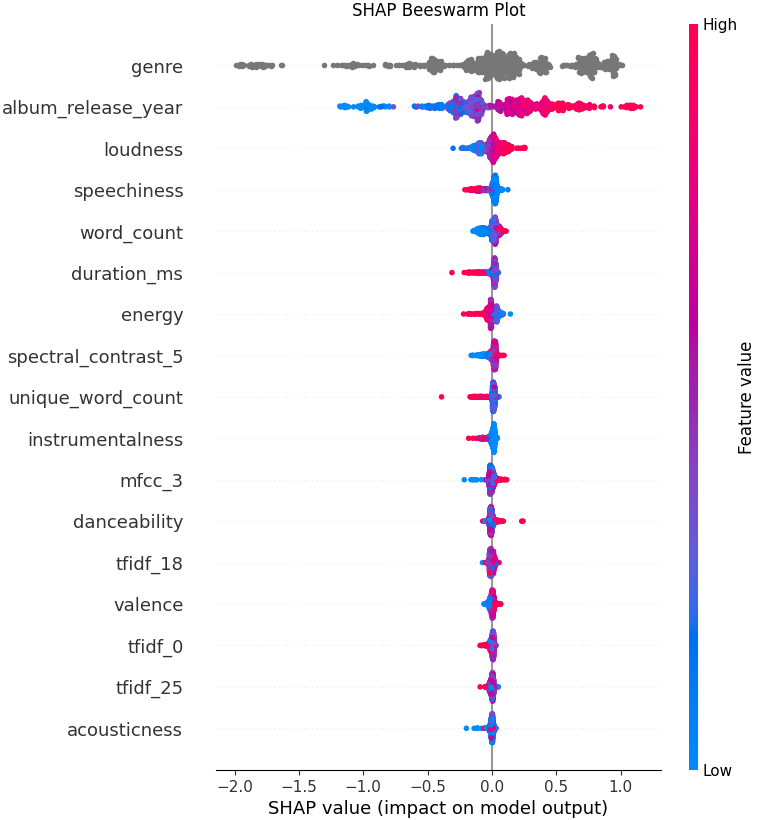
\includegraphics[width=5in]{img/beeswarm_popularity_reg.png}
  \caption{SHAP beeswarm plot of the regression model for popularity trained on all features.}
  \label{Figure:fig_beh}
\end{figure}
\end{center}

\begin{itemize}
  \item Higher values of \textit{Release Year} strongly correlate with higher
    \textit{Popularity}, indicating that newer songs are generally more
    popular.
  \item Higher \textit{loudness} and lower \textit{speechiness}
    were associated with increased \textit{popularity}, reflecting their
    influence on listener preferences and music trends.
\end{itemize}



%---------------------------------------------------------------------------
\subsection{Classification Approach}

The task of predicting song popularity was reformulated as a binary
classification problem, where the target was to determine whether a song is
"popular" (1) or "not popular" (0). In order to create those labels from an
integer variable with range 0-100, the \textbf{70th perrcentile of the
popularity values was used as the threshold}. Songs with popularity greater or
equal  than this  threshold werre  labeled as popular, and the rest was labeled
as unpopular. This thresholding approach based on quantile ensures a balanced
representation of popular songs in the dataset while accounting for the
naturally skewed distribution of  popularity scores.

% \usepackage{tabularray}
\begin{table}[H]
\centering
\caption{Results of classification of popularity.}
\begin{tblr}{
  hline{2} = {-}{},
}
 & \textbf{Model}          & \textbf{Features} & \textbf{Accuracy} & \textbf{F1(w.avg.)} \\
 & Baseline Majority Model &                   & 65.93\%           & 52.39\%             \\
 & Baseline Random Model   &                   & 48.27\%           & 49.57\%             \\
 & Catboost                & all               & \textbf{84.68\%}  & \textbf{84.71\%}    \\
 & Catboost                & lyrical           & 65.79\%           & 64.77\%             \\
 & Catboost                & spotify data      & \textbf{82.06\%}  & \textbf{82.32\%}    \\
 & Catboost                & audio             & 63.17\%           & 63.00\%             
\end{tblr}
\end{table}


The classification models were evaluated using accuracy and weighted F1-score.
\textit{Baseline Majority Model} (which predicts the majority class for all
samples) achieved an accuracy of 65.93\% and an F1-score of 52.39\%. This
reflects the class imbalance introduced by the thresholding, with a higher
proportion of songs being labeled as "not popular."

The \textit{Baseline Random Model}, which guesses classes randomly, performed
worse in accuracy (48.27\%) and achieved a slightly higher F1-score of 49.57\%
compared to accuracy due to its balanced attempts to handle both classes.

The CatBoost model significantly outperformed both baselines, achieving an
overall accuracy of 84.68\% and a weighted F1-score of 84.71\% when trained on
all features.This result demonstrates the effectiveness of the full feature set
in capturing the complexity of popularity prediction.


The CatBoost model trained on Spotify data performed well, with an accuracy of
82.06\% and an F1-score of 82.32\%, showing that Spotify features alone provide
strong predictive power. However, the model trained on all features slightly
surpassed it, suggesting that additional features offer some complementary
information.

The model using only lyrical features achieved an accuracy of 65.79\%, lower
than the \textit{Baseline Majority Model}, but a higher F1-score of 64.77\%,
reflecting its ability to handle class imbalance better than the majority
model. This confirms that lyrical features are limited in their ability to
predict song popularity.


The performance of the model trained on features extracted from audio files was
similar to the lyrical one, demonstrating that isolated audio features are not
sufficient to fully predict popularity.


SHAP analysis revealed that key features such as \textit{genre}, \textit{album
release year} and \textit{loudness} were the most
significant predictors of popularity. These findings were consistent with the
regression task, reinforcing the robustness of these features across different
modeling approaches. This consistency highlights their central role in
understanding and predicting song success.


\begin{center}
\begin{figure}[H]
  \centering
  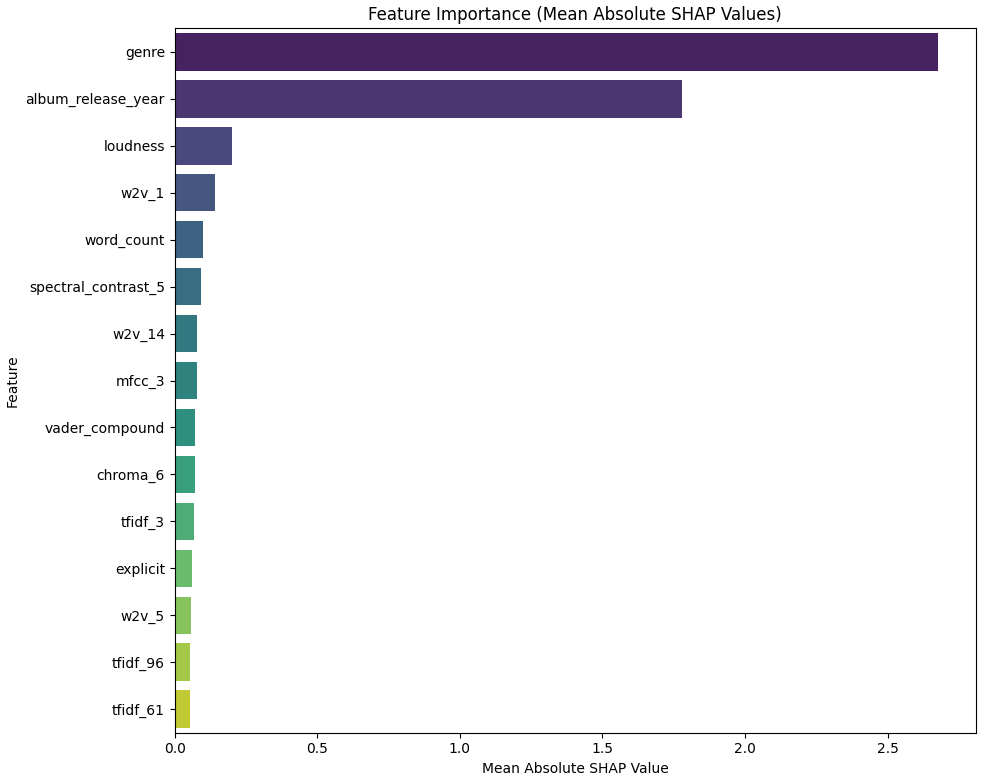
\includegraphics[width=5in]{img/feature_importance_popularity_clf.png}
  \caption{SHAP feature importance plot of the classification model for popularity trained on all features.}
  \label{Figure:fig_beh}
\end{figure}
\end{center}

\begin{center}
\begin{figure}[H]
  \centering
  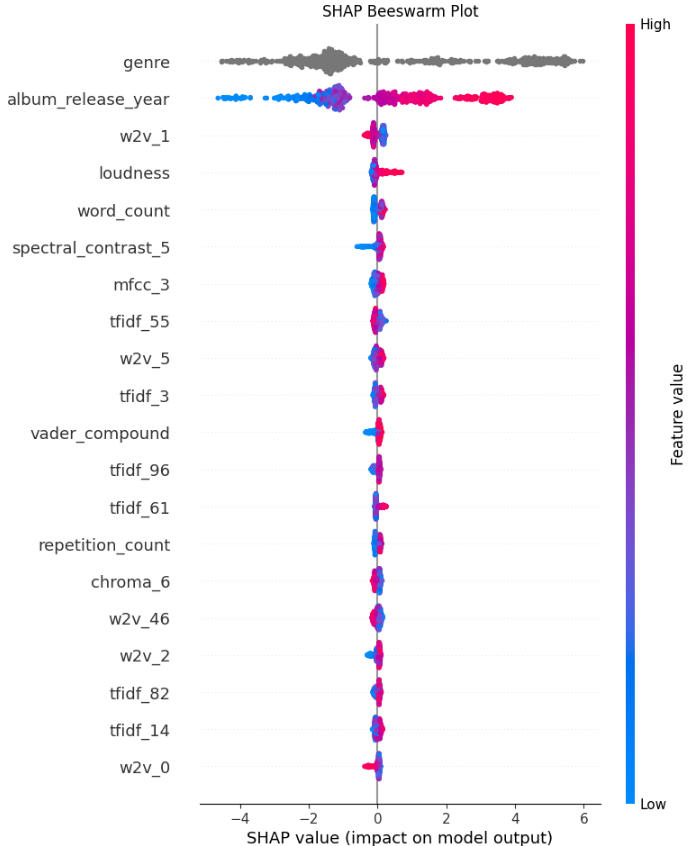
\includegraphics[width=5in]{img/beeswarm_popularity_clf.png}
  \caption{SHAP beeswarm plot of the classification model for popularity trained on all features.}
  \label{Figure:fig_beh}
\end{figure}
\end{center}



The SHAP analysis for the classification model highlights similar dependencies
to the regression model. Key features like \textit{genre} and
\textit{album release year} remain the most important, emphasizing their role
in shaping song popularity. 

Several differences can be observed between feature importance in the
regression and classification model, notably:
\begin{itemize}
  \item Lyrics embeddings(TF-IDF and Word2Vec) seemed to play a bigger role in
    the classification model.
  \item Classification model seemed to pay much less attention to Spotify audio
    features, like \textit{danceability}, \textit{energy} and
    \textit{speechiness}.
  \item Unlike in regression, in classification a sentiment metric,
    \textit{VADER compound} contributed to the prediction of popularity. More
    popular songs tend to have more positive lyrics.
\end{itemize}


%---------------------------------------------------------------------------
\section{Explicitness}
\label{sec:explicitness}

\subsection{Classification Approach}
The task of predicting whether a song contains explicit content was approached
as a classification problem. The performance of the CatBoost model was compared
against baseline on different feature subsets. One of the key challenges of
this problem was significant class imbalance present in the dataset;
approximately 85\% of the songs did not contain explicit content.

Significant class imbalance can lead to models favoring the majority class,
potentially resulting in  high accuracy but poor performance on the minority
class. To address this problem, CatBoost's class weights parameter was used.
This parameter allowed the model to penalize misclassifications of the minority
class more heavily, therefore improving its ability to recognize explicit
content.

% \usepackage{tabularray}
\begin{table}[H]
\centering
\caption{Results of classification of explicitness.}
\begin{tblr}{
  hline{2} = {-}{},
}
 & \textbf{Model}          & \textbf{Features} & \textbf{Accuracy} & \textbf{F1 weighted average} \\
 & Baseline Majority Model &                   & 84.00\%           & 76.69\%                      \\
 & Baseline Random Model   &                   & 47.03\%           & 53.91\%                      \\
 & Catboost                & all               & \textbf{92.41\%}  & \textbf{92.40\%}             \\
 & Catboost                & lyrical           & \textbf{92.41\%}  & \textbf{92.25\%}             \\
 & Catboost                & spotify data      & 86.48\%           & 87.11\%                      \\
 & Catboost                & audio             & 82.75\%           & 82.47\%                      
\end{tblr}
\end{table}


The table presents the results of the models in terms of accurracy and weighted
F1 score. The \textit{Baseline Majority Model} achieved accuracy of 84\% and
significantly lower F1 weighted average of 76.69\%, which reflects its inability
to handle class balance effectively. The \textit{Baseline Random Model}
performed very poorly, with an accuracy of 47.03\% and F1 weighted average of
53.91\%.

In contrast, the CatBoost model outperformed both baselines achieving accuracy
of \textbf{92.41\%} and weighted average score of \textbf{92.4\%} when trained
on all features. Interestingly, the model trained only using lyrical features
performed nearly as well, indicating that explicitness can largely be predicted
based on lyrical content. Models that relied on Spotify metadata and features
extracted from audio files had lower performance, achieving accurracy close to
\textit{Baseline Majority Model}, but with higher F1 scores, due to their
ability to address class imbalance. These observations emphasize the centrality
of lyrical information in prediction of explicit content.


\begin{center}
\begin{figure}[H]
  \centering
  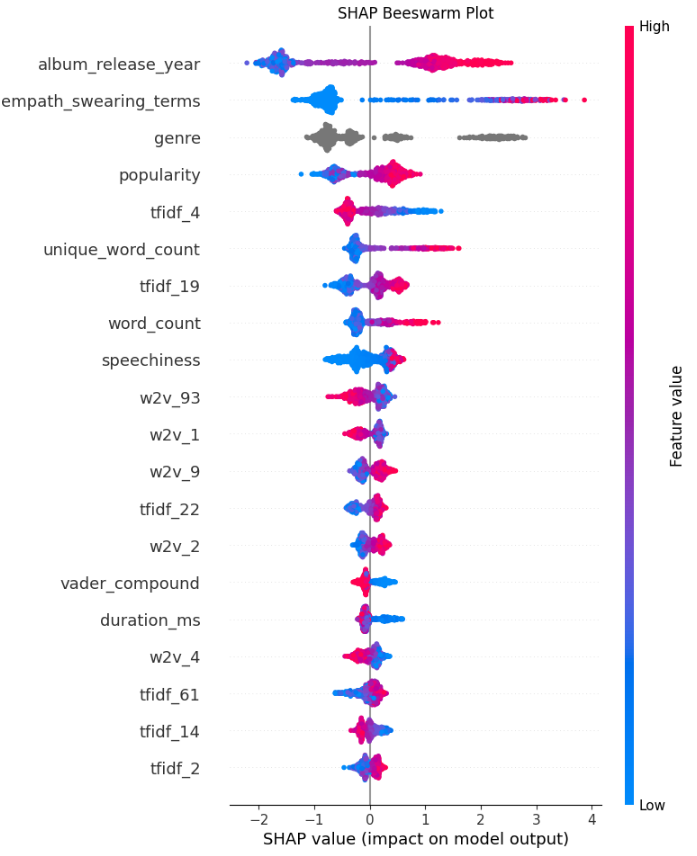
\includegraphics[width=5in]{img/beeswarm_explicitness.png}
  \caption{SHAP beeswarm plot of the classification model for explicitness trained on all features.}
  \label{Figure:fig_beh}
\end{figure}
\end{center}

\begin{center}
\begin{figure}[H]
  \centering
  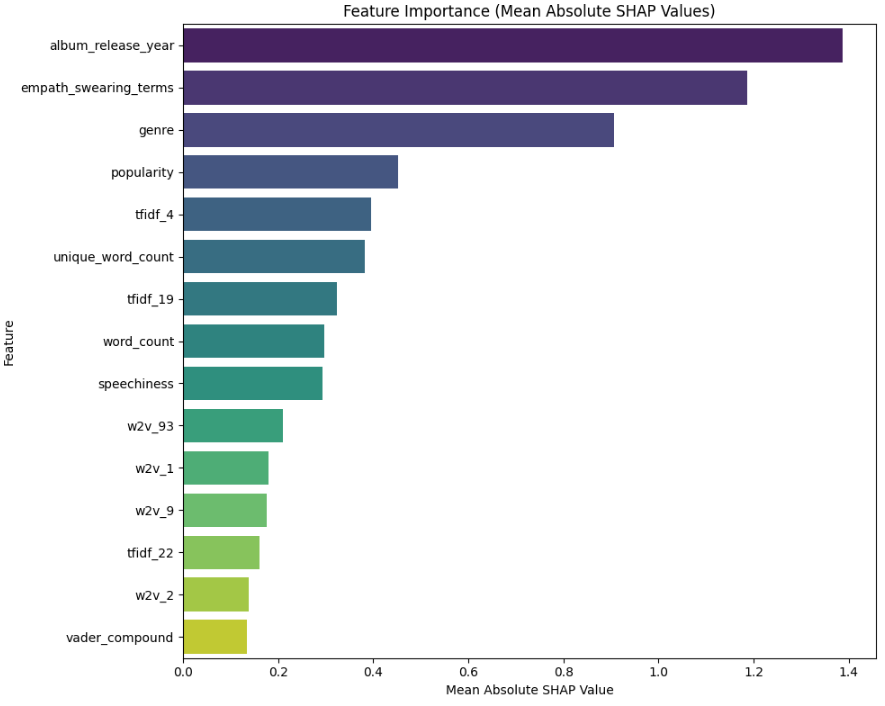
\includegraphics[width=5in]{img/feature_importance_explicitness.png}
  \caption{SHAP beeswarm plot of the classification model for explicitness  trained on all features.}
  \label{Figure:fig_beh}
\end{figure}
\end{center}


Based on the SHAP analysis we can observe that the key features for this task
turned out to be:
\begin{itemize}
  \item \textbf{Album Release Year}: this feature had  highest feature
    importance, reflecting temporal trends in explicit content. Newer songs are
    statistically more likely to contain explicit language, reflecting changing
    societal norms and artistic expressions over time.
  \item \textbf{Empath Swearing Terms}: As expected, the presence of swearing
    terms was a strong indicator of explicitness.
  \item \textbf{Genre} was the third most important feature, showing that
    certain genres  are more likely to contain explicit content than others.
  \item \textbf{TF-IDF}: several vectors created using TF-IDF and later reduced
    via PCA significantly contributed to the model's predictions. Similar to
    the Empath feature, TF-IDF likely captured swear words and related patterns
    in the lyrics, reinforcing its importance.
  \item \textbf{Speechiness}: songs with higher values of
    speechiness—indicating a greater presence of spoken-word elements—were more
    likely to be labeled as explicit.
\end{itemize}




The task of predicting explicitness could potentially achieve higher
performance by leveraging the interpretability of explicitness, which provides
clear hints about the most relevant features for this property. However, the
primary goal of this analysis was not to maximize model performance but to
explore the impact of various feature subsets on the prediction of
explicitness.

The results indicate that predicting explicitness based solely on audio
features is inherently challenging. The model trained on audio features
performed worse than the baseline, suggesting that the extracted audio
characteristics from the MP3 files do not sufficiently capture the explicit
nature of songs. This highlights the need for features more directly related to
lyrical or contextual information when modeling explicit content.



%---------------------------------------------------------------------------
\subsection{Impact of Explicit Language on Popularity and Sentiment}
\label{sec:explicitmorepopular}

The relationship between explicit content and song popularity is a topic of
interest in understanding the cultural and commercial dynamics of music.
Explicit songs often reflect bold themes, which may resonate more strongly with
certain audiences. 

To investigate this, a bootstrap test was conducted to determine whether
explicit songs are, on average, more popular than non-explicit songs. Bootstrap
was chosen for this analysis due to its robustness and flexibility. Unlike
traditional parametric tests, the bootstrap method does not rely on strong
assumptions about the underlying data distribution, making it well-suited for
analyzing real-world datasets that may not meet normality or other strict
requirements.


\begin{center}
\begin{figure}[H]
  \centering
  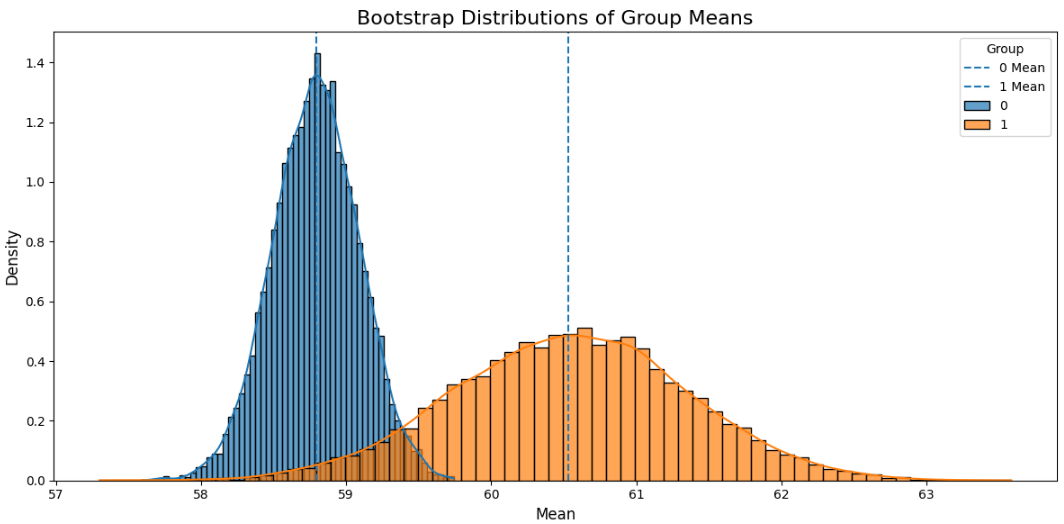
\includegraphics[width=5in]{img/explicitness_bootstrap.png}
  \caption{Bootstrap Test to check if explicit songs are on average more
  popular.}
  \label{Figure:fig_bh}
\end{figure}
\end{center}



\begin{center}
\begin{figure}[H]
  \centering
  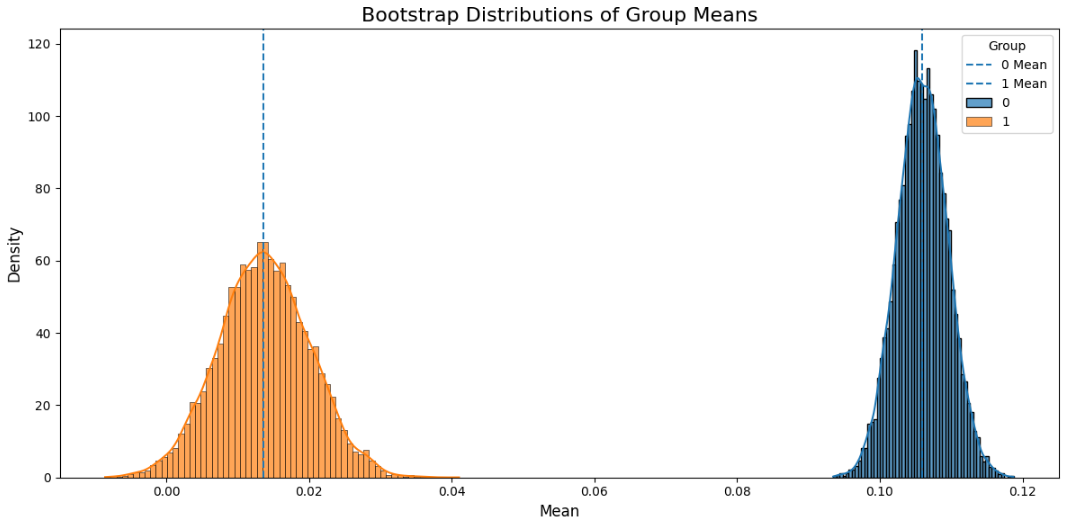
\includegraphics[width=5in]{img/explicitness_bootstrap_2.png}
  \caption{Bootstrap Test to check if explicit songs are on average more
  positive or negative than non-explicit songs.}
  \label{Figure:fig_bh}
\end{figure}
\end{center}



\begin{table}[H]
\centering
\caption{Results of the Bootstrap Test.}
\resizebox{\linewidth}{!}    & 0.08\%                  & 5.79\%                           & 1.74               & 0.0453                        & 3.4013                        \\
Sentiment~ Polarity & non-explicit           & explicit                 & \textbf{-87.10\%}  & -100.69\%               & -73.63\%                         & -0.09              & -0.1067                       & -0.0780                       
\end{tblr}
}
\end{table}


The analysis reveals that explicit songs are, on average, \textbf{2.96\% more
popular} than non-explicit songs. The confidence interval of [0.08\%, 5.79\%]
suggests statistically significant but modest increase in popularity for
explicit songs.

For sentiment polarity, explicit songs turned out to be on average
\textbf{87.10\% less positive} than non-explicit songs. The confidence interval
of [-100.69\%, -73.63\%] suggests a very significant difference. This
observation aligns with the notion that bold songs that contain explicit
language often reflect intense or provocative themes, which may carry less
positive emotion.

%---------------------------------------------------------------------------
\section{Sentiment}
\label{sec:sentiment}

This section tackles the problem of song lyrics sentiment prediction. The
binary sentiment labels(positive (1) and negative (0)) were derived from the
variable \textit{sentiment polarity}. Songs with polarity values below 0 were
labeled as negative, while those above 0 were labeled as positive.

This process resulted in an unbalanced target variable, where the positive
class was overrepresented. Additionally, due to the left-skewed distribution of
\textit{sentiment polarity}, songs labeled as \textit{positive} were, on
average, more strongly positive compared to the relatively moderate negativity
of songs in the \textit{negative} class.

While this imbalance and class definition might pose challenges for traditional
predictive modeling, it is not a major concern for this study. The primary
objective is to understand which factors contribute to a song's sentiment
rather than achieving perfect predictive accuracy. Chosen approach
provides sufficient insight into the relationship between song features and
sentiment.



\begin{table}[H]
\centering
\caption{Results of classification of sentiment.}
\begin{tblr}{
  hline{2} = {-}{},
}
 & \textbf{Model}          & \textbf{Features} & \textbf{Accuracy} & \textbf{F1(w.avg.)} \\
 & Baseline Majority Model &                   & 69.65\%           & 57.19\%             \\
 & Baseline Random Model   &                   & 52.55\%           & 54.46\%             \\
 & Catboost                & all               & 71.44\%           & 69.77\%             \\
 & Catboost                & lyrical           & \textbf{71.86\%}  & \textbf{70.72\%}    \\
 & Catboost                & spotify data      & 67.44\%           & 64.94\%             \\
 & Catboost                & audio             & 65.10\%           & 63.43\%             
\end{tblr}
\end{table}




The \textit{Baseline Majority Model}, which simply predicted the most common
class for all samples, achieved an accuracy of 69.65\% and an F1-score of
57.19\%, reflecting the class imbalance in the dataset. The \textit{Baseline
Random Model}, which predicted classes randomly, performed worse in terms of
accuracy (52.55\%) but slightly better in F1-score (54.46\%).

Among the CatBoost models, the one trained solely on lyrical features performed
the best, achieving an accuracy of 71.86\% and a weighted F1-score of 70.72\%.
This highlights the importance of lyrical features in capturing sentiment. The
model trained on all features followed closely, but performed slightly worse
due to large amount of redundant features, despite the presence of feature
selection step in the pipeline that attempted to discard them.

Models trained on only Spotify or audio features performed worse, achieving
accuracies of 67.44\% and 65.10\%, respectively. These results suggest that
while Spotify and audio features capture useful information, they are less
indicative of sentiment compared to lyrical data. 

The results indicate that features extracted directly from MP3 files are not
strong predictors of a song's sentiment, despite the intuitive assumption that
audio characteristics should play a role. This outcome suggests that the
current set of extracted audio features may not sufficiently capture the
nuanced aspects of sentiment. Future work could focus on advanced feature
engineering or exploring additional audio-based descriptors to improve the
performance of audio-based sentiment prediction models.

\begin{center}
\begin{figure}[H]
  \centering
  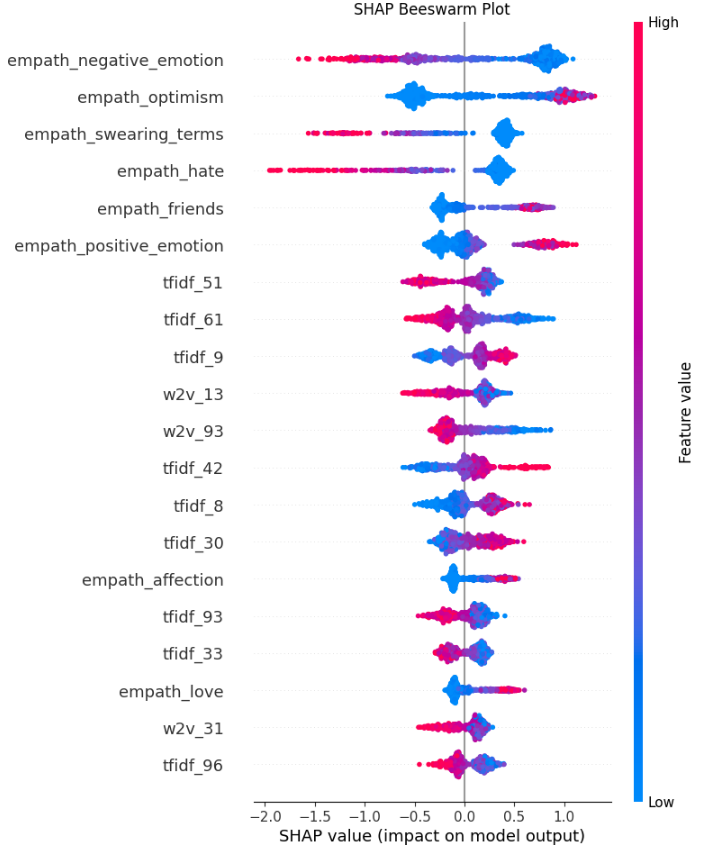
\includegraphics[width=5in]{img/beeswarm_sentiment.png}
  \caption{SHAP beeswarm plot of the classification model for sentiment
  trained on all features.}
  \label{Figure:fig_bh}
\end{figure}
\end{center}

\begin{center}
\begin{figure}[H]
  \centering
  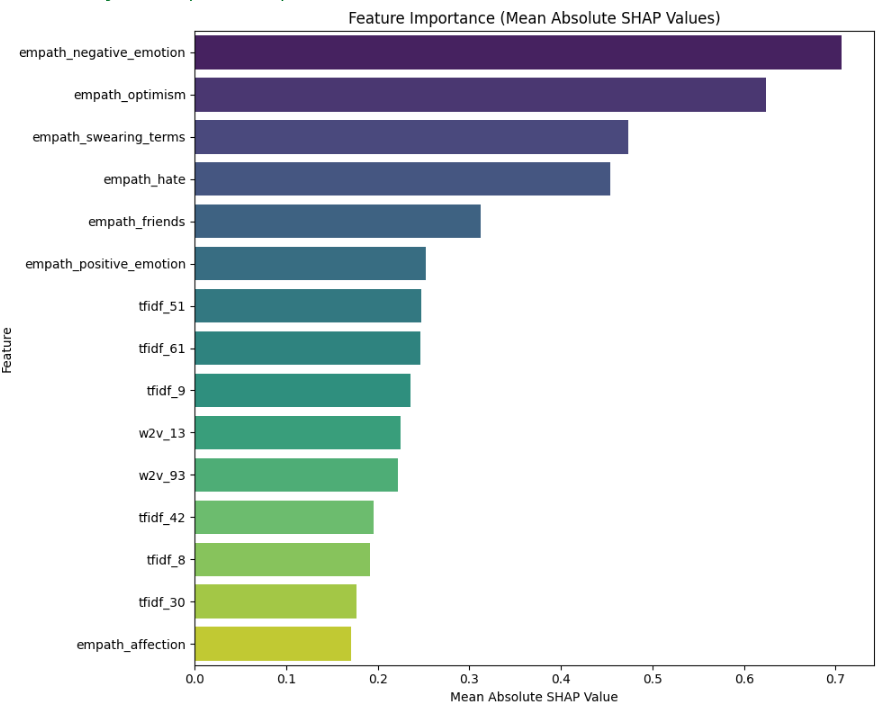
\includegraphics[width=5in]{img/feature_importance_sentiment.png}
  \caption{SHAP feature importance plot of the classification model for
  sentiment trained on all features.}
  \label{Figure:fig_eh}
\end{figure}
\end{center}

The SHAP analysis showed that lyrical features, like empath_negative_emotion,
empath_optimism, and empath_swearing_terms, were the most influential in
predicting sentiment, with negative emotions and swearing linked to negative
sentiment, and optimism and positive emotion tied to positive sentiment. TF-IDF
and Word2Vec embeddings also contributed, reflecting patterns in lyrics. Audio
features, however, had minimal impact, emphasizing the need for improved audio
feature engineering to capture sentiment.

%---------------------------------------------------------------------------
